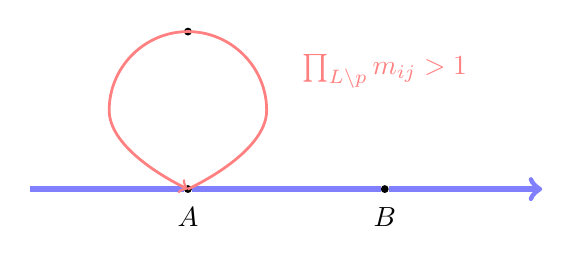
\begin{tikzpicture}[node distance=10pt]
\tikzstyle{blackdot} = [circle,fill, scale=0.3];
\node [blackdot] (v1) at (-1.5,0.5) {};
\node [below of=v1] {$A$};
\node [blackdot] (v2) at (1,0.5) {};
\node [below of=v2] {$B$};
\draw[->,line width=2pt,blue!50] (-3.5,0.5) -- (v1) -- (v2) -- (3,0.5);
\node [blackdot] (v3) at (-1.5,2.5) {};
\draw[->,line width=1pt,red!50]  plot[smooth, tension=.99] coordinates {(v1) (-0.5,1.5) (v3) (-2.5,1.5) (-1.5,0.5)};
\node[red!50] at (1,2) {$\prod_{L\backslash p}m_{ij}>1$};
\end{tikzpicture}
